\section{Device and Process Integration}
HBM DRAM stacks are typically fabricated with high-temperature capacitor anneals ($>700~^\circ$C),
whereas FeRAM/FeFET devices require lower-temperature processing ($\sim$400~^\circ$C$) to stabilize the ferroelectric o-phase in HfO$_2$.
This thermal budget mismatch currently hinders monolithic integration.

\subsection{Chiplet-based Integration (Practical Solution)}
The most practical near-term approach is chiplet-based integration:
HBM stacks and FeRAM/FeFET dies are fabricated in their respective optimized flows and co-integrated on a silicon interposer using $\mu$-bump connections.
This architecture enables:
\begin{itemize}
  \item High-bandwidth operation from HBM ($>$300~GB/s),
  \item Persistent storage of checkpoints, metadata, and cold data in FeRAM,
  \item Reduction of refresh-induced traffic in DRAM.
\end{itemize}

\subsection{Monolithic Integration (Research Challenge)}
A longer-term research direction is embedding FeFET arrays within the HBM logic base die.
In principle, DRAM capacitor HfO$_2$ and FeFET gate-stack HfO$_2$ could coexist; however, their annealing requirements remain incompatible.
Potential enablers include selective or dual-step annealing, dopant modulation, or stress engineering.
At present, monolithic HBM+FeFET integration remains an open challenge for device and process research.

% ===== Fig.1: Minimal chiplet integration(座標固定で重なり解消) =====
\begin{figure}[t]
\centering
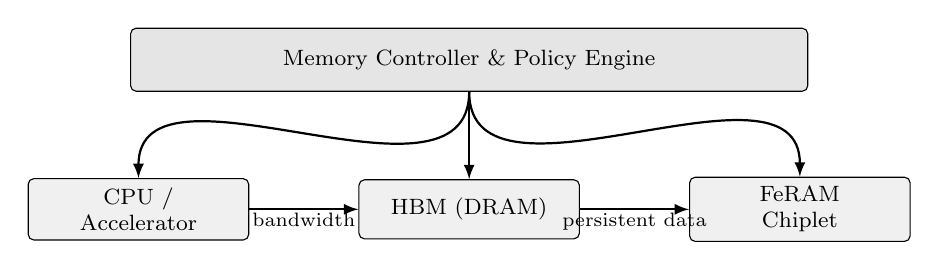
\begin{tikzpicture}[
  font=\footnotesize, >=latex, x=1cm, y=1cm,
  box/.style={draw, rounded corners=2pt, fill=black!6,
              minimum width=28mm, minimum height=7.5mm, align=center},
  ctrl/.style={draw, rounded corners=2pt, fill=black!10,
               minimum width=86mm, minimum height=8mm, align=center}
]

% 上段コントローラ(y=1.9)
\node[ctrl] (mc) at (0,1.9) {Memory Controller \& Policy Engine};

% 下段3ブロック(y=0)— 間隔を広めに x= -4.2, 0, +4.2
\node[box] (cpu)   at (-4.2,0) {CPU /\\ Accelerator};
\node[box] (hbm)   at ( 0.0,0) {HBM (DRAM)};
\node[box] (feram) at ( 4.2,0) {FeRAM\\ Chiplet};

% データパス(下段同士)
\draw[->, thick] (cpu) -- node[midway, below, inner sep=1pt]{\scriptsize bandwidth} (hbm);
\draw[->, thick] (hbm) -- node[midway, below, inner sep=1pt]{\scriptsize persistent data} (feram);

% コントローラからの制御線(曲げて重なり防止)
\draw[->, thick] (mc.south) to[out=-90,in=90] (cpu.north);
\draw[->, thick] (mc.south) -- (hbm.north);
\draw[->, thick] (mc.south) to[out=-90,in=90] (feram.north);

\end{tikzpicture}

\vspace{3pt}
\caption{Minimal chiplet integration view. CPU$\rightarrow$HBM は帯域を供給し,
永続データとチェックポイントは FeRAM チップレットに保持。
上段のコントローラ/ポリシーエンジンが tiering と checkpointing を統括する。}
\label{fig:chiplet_min}
\end{figure}
